%% Auto-generated by scripts/generate_figures.py
\begin{figure}[htbp]
\centering
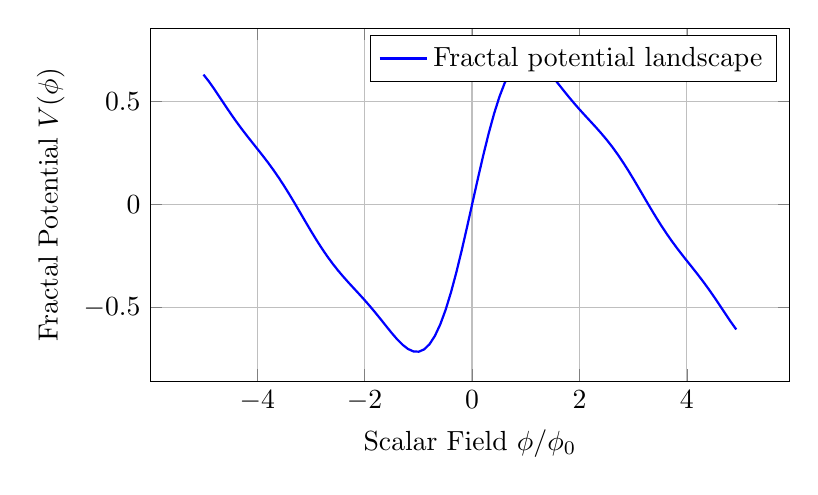
\begin{tikzpicture}
  \begin{axis}[
    width=0.8\textwidth,
    height=0.5\textwidth,
    xlabel={Scalar Field $\phi / \phi_0$},
    ylabel={Fractal Potential $V(\phi)$},
    grid=major
  ]
    \addplot[blue, thick] coordinates {
      (-5.0000, 6.315410e-01)
      (-4.8998, 5.983945e-01)
      (-4.7996, 5.613401e-01)
      (-4.6994, 5.223067e-01)
      (-4.5992, 4.828656e-01)
      (-4.4990, 4.441590e-01)
      (-4.3988, 4.068708e-01)
      (-4.2986, 3.712403e-01)
      (-4.1984, 3.371154e-01)
      (-4.0982, 3.040358e-01)
      (-3.9980, 2.713395e-01)
      (-3.8978, 2.382789e-01)
      (-3.7976, 2.041348e-01)
      (-3.6974, 1.683190e-01)
      (-3.5972, 1.304530e-01)
      (-3.4970, 9.041855e-02)
      (-3.3968, 4.837417e-02)
      (-3.2966, 4.737886e-03)
      (-3.1964, -3.986045e-02)
      (-3.0962, -8.465177e-02)
      (-2.9960, -1.288164e-01)
      (-2.8958, -1.715784e-01)
      (-2.7956, -2.122955e-01)
      (-2.6954, -2.505331e-01)
      (-2.5952, -2.861151e-01)
      (-2.4950, -3.191438e-01)
      (-2.3948, -3.499865e-01)
      (-2.2946, -3.792284e-01)
      (-2.1944, -4.075956e-01)
      (-2.0942, -4.358553e-01)
      (-1.9940, -4.647013e-01)
      (-1.8938, -4.946378e-01)
      (-1.7936, -5.258721e-01)
      (-1.6934, -5.582277e-01)
      (-1.5932, -5.910884e-01)
      (-1.4930, -6.233806e-01)
      (-1.3928, -6.535979e-01)
      (-1.2926, -6.798690e-01)
      (-1.1924, -7.000652e-01)
      (-1.0922, -7.119405e-01)
      (-0.9920, -7.132949e-01)
      (-0.8918, -7.021467e-01)
      (-0.7916, -6.769019e-01)
      (-0.6914, -6.365050e-01)
      (-0.5912, -5.805590e-01)
      (-0.4910, -5.094042e-01)
      (-0.3908, -4.241469e-01)
      (-0.2906, -3.266357e-01)
      (-0.1904, -2.193849e-01)
      (-0.0902, -1.054493e-01)
      (0.0100, 1.173922e-02)
      (0.1102, 1.285644e-01)
      (0.2104, 2.414303e-01)
      (0.3106, 3.469660e-01)
      (0.4108, 4.422124e-01)
      (0.5110, 5.247796e-01)
      (0.6112, 5.929626e-01)
      (0.7114, 6.458079e-01)
      (0.8116, 6.831263e-01)
      (0.9118, 7.054539e-01)
      (1.0120, 7.139645e-01)
      (1.1122, 7.103424e-01)
      (1.2124, 6.966265e-01)
      (1.3126, 6.750399e-01)
      (1.4128, 6.478175e-01)
      (1.5130, 6.170469e-01)
      (1.6132, 5.845340e-01)
      (1.7134, 5.517029e-01)
      (1.8136, 5.195364e-01)
      (1.9138, 4.885604e-01)
      (2.0140, 4.588689e-01)
      (2.1142, 4.301880e-01)
      (2.2144, 4.019663e-01)
      (2.3146, 3.734860e-01)
      (2.4148, 3.439794e-01)
      (2.5150, 3.127411e-01)
      (2.6152, 2.792242e-01)
      (2.7154, 2.431114e-01)
      (2.8156, 2.043560e-01)
      (2.9158, 1.631885e-01)
      (3.0160, 1.200897e-01)
      (3.1162, 7.573530e-02)
      (3.2164, 3.091729e-02)
      (3.3166, -1.354721e-02)
      (3.4168, -5.691020e-02)
      (3.5170, -9.857901e-02)
      (3.6172, -1.381845e-01)
      (3.7174, -1.756230e-01)
      (3.8176, -2.110674e-01)
      (3.9178, -2.449427e-01)
      (4.0180, -2.778707e-01)
      (4.1182, -3.105847e-01)
      (4.2184, -3.438249e-01)
      (4.3186, -3.782221e-01)
      (4.4188, -4.141827e-01)
      (4.5190, -4.517869e-01)
      (4.6192, -4.907094e-01)
      (4.7194, -5.301747e-01)
      (4.8196, -5.689514e-01)
      (4.9198, -6.053895e-01)
    };
    \addlegendentry{Fractal potential landscape}
  \end{axis}
\end{tikzpicture}
\caption{Representative fractal modulated scalar potential spanning multiple resonant scales.}
\label{fig:fractal-potential}
\end{figure}
